\begin{figure}[ht!]
\centering
% manually adjust the width of the figure
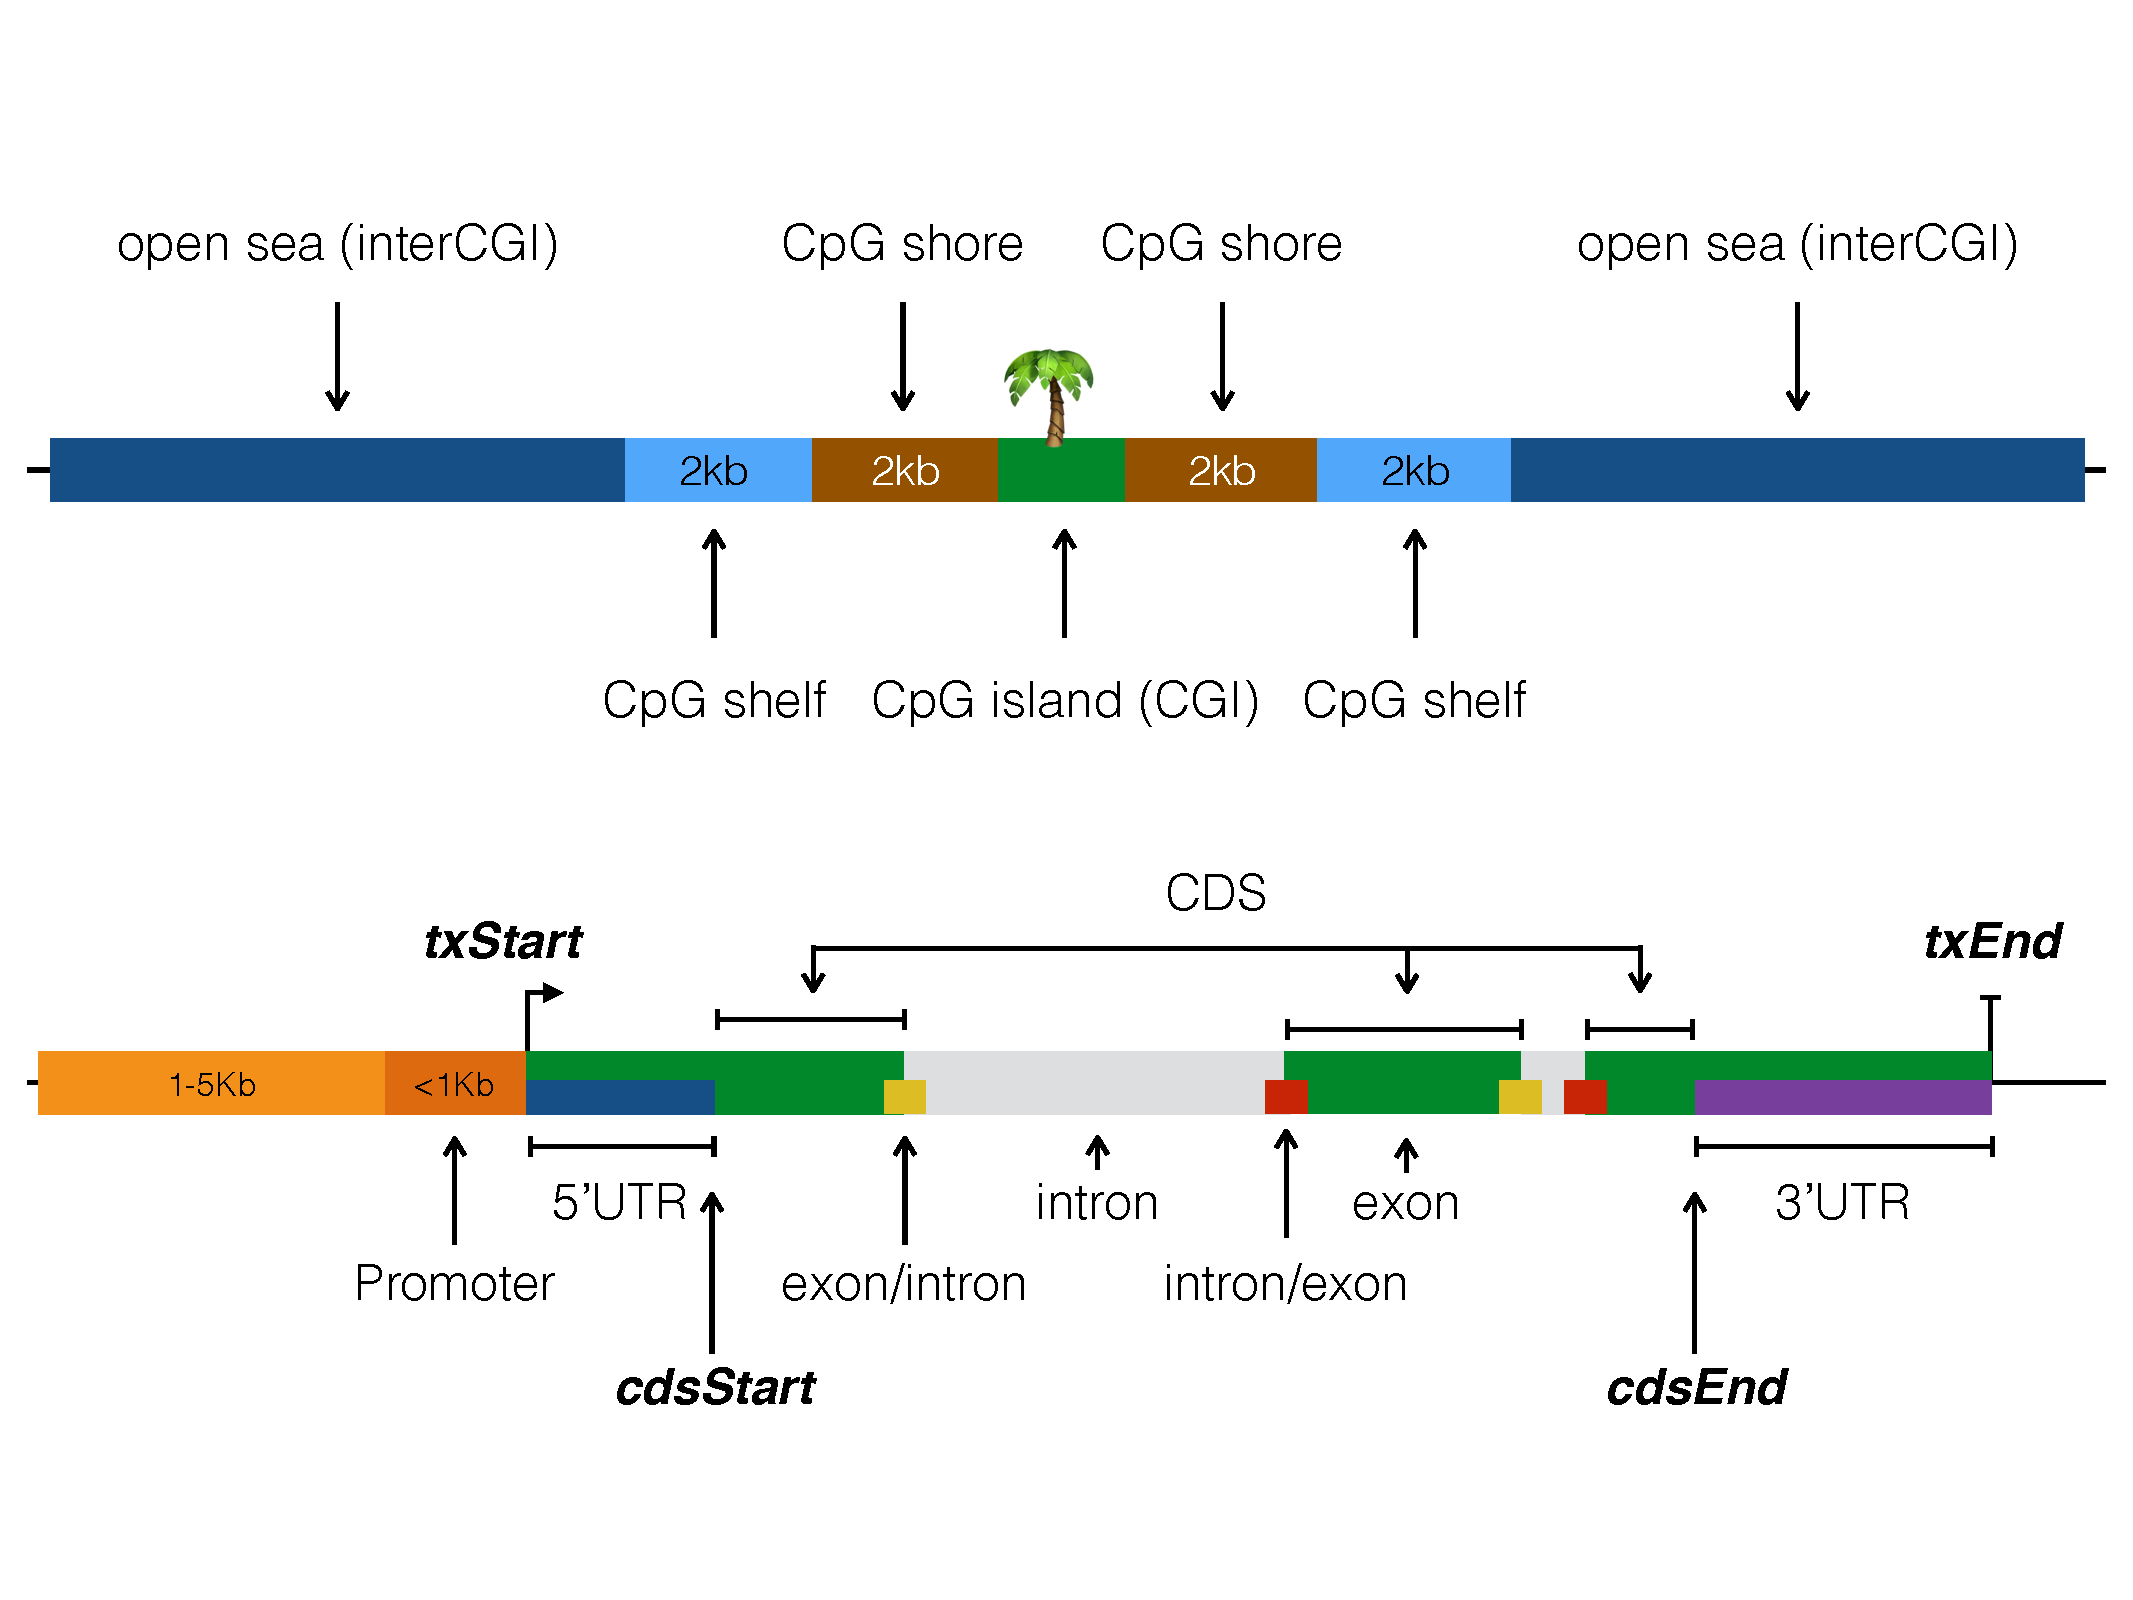
\includegraphics[width=1\textwidth]{chap4figs/figure4_1.pdf}
\caption[Schematics of the CpG and genic annotation types used.]
{
% Rackham requires the figure list title matches the first sentence, so repeat that sentence here
\textbf{Schematics of the CpG and genic annotation types used.} (Top) Schematic of the UCSC CpG annotations used in annotatr. The CpG islands are retrieved from either the AnnotationHub R package or the UCSC Golden Path, depending on availability for the genome build. CpG shores are defined as the 2kb extension upstream and downstream of the CpG island boundaries, less any CpG islands. The CpG shelves are a further 2kb extension upstream and downstream of the furthest upstream and downstream boundaries of the CpG shores, less any CpG island and shore annotations. The complement of the CpG islands, shores, and shelves make up the "open sea" or interCGI annotation. (Bottom) A schematic of the genic annotations available in annotatr. Functions from the GenomicFeatures R package in conjunction with custom functions are used to extract regions 1-5Kb upstream of a TSS, promoters, 5'UTRs, exons, introns, and 3'UTRs. Additionally, exon/intron and intron/exon boundaries are determined by 200bp regions around such boundaries. Annotations may overlap one another from the same or from different transcripts. Genic annotations always have UCSC Transcript IDs and Entrez Gene IDs and gene symbols when applicable.
}
\label{chap4:fig:1}
\end{figure}

\newpage

\begin{figure}[!ht]

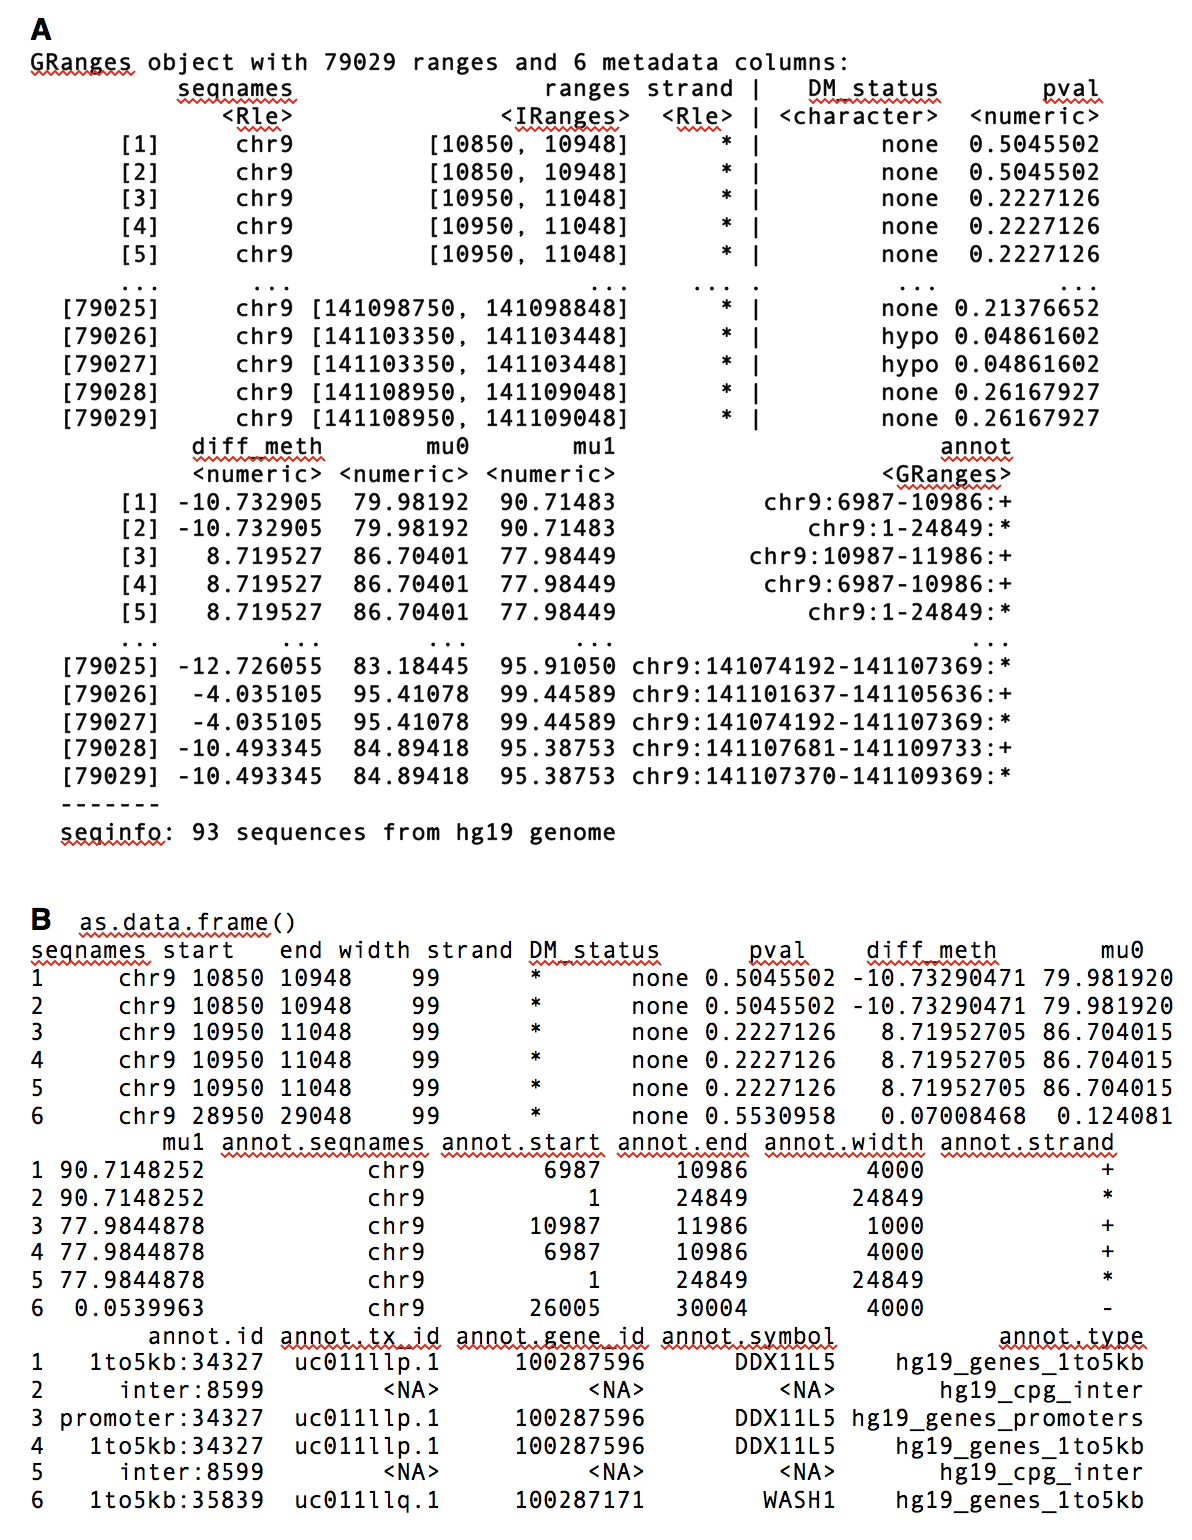
\includegraphics[width=0.8\textwidth]{chap4tables/table4_3.png}
\caption[Example output of the annotate\_regions() function as a GRanges object (A) and data.frame (B).]
{
% Rackham requires the figure list title matches the first sentence, so repeat that sentence here
\textbf{Example output of the annotate\_regions() function as a GRanges object (A) and data.frame (B).}
(A) Output of GRanges object with extra columns containing extra data from the input regions (DM\_status, pval, diff\_meth, mu0, and mu1). In addition, a column giving complete details about the annotations is in the annot column, however the gene information is hidden in this output. Of note is that regions with multiple annotations are repeated (see rows 1-2 and 3-5). (B) Using data.frame() allows users to coerce this GRanges object into a flat table and expose the gene information (last five columns).
}
\label{chap4:table:3}

\end{figure}

\newpage

\begin{figure}[ht!]
\centering
% manually adjust the width of the figure
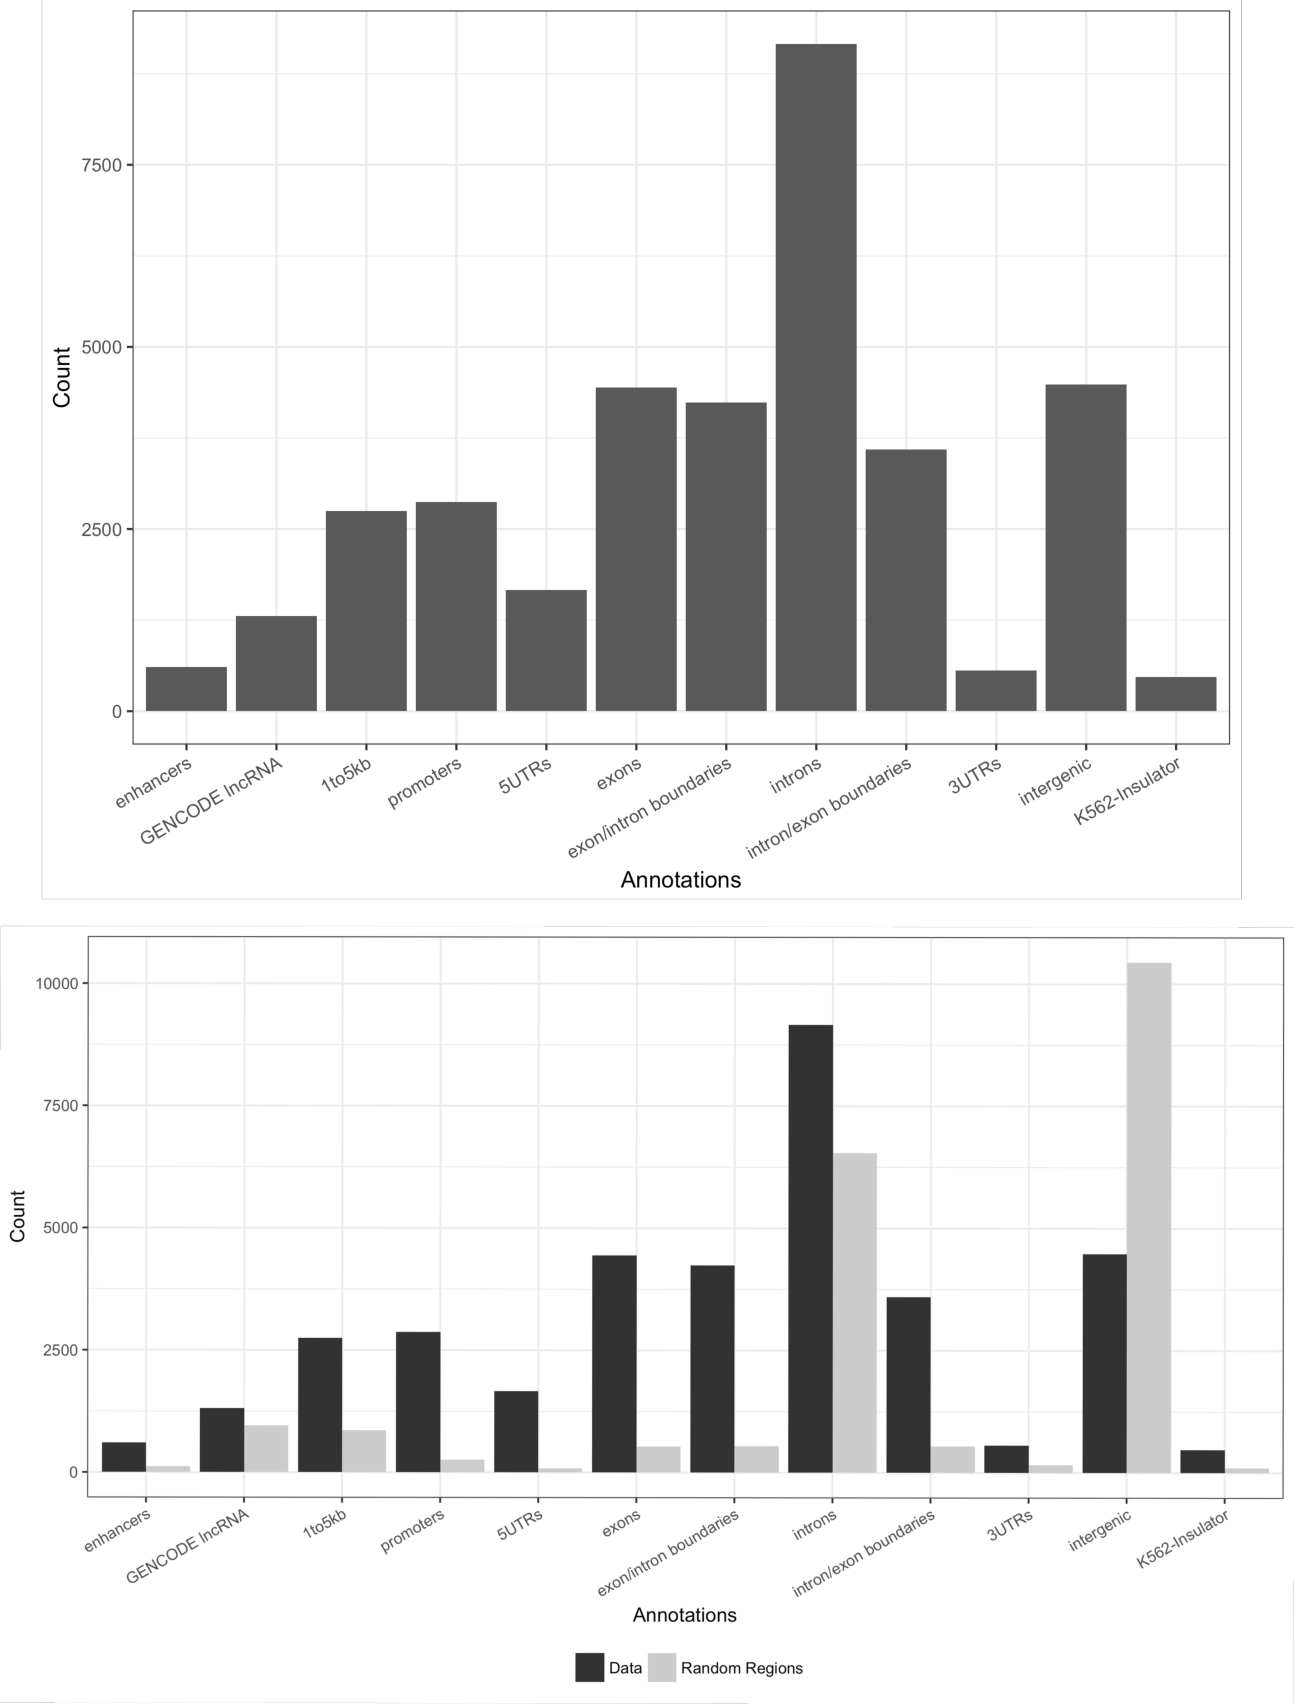
\includegraphics[width=1\textwidth]{chap4figs/figure4_2.pdf}
\caption[Examples of annotatr barplots.]
{
% Rackham requires the figure list title matches the first sentence, so repeat that sentence here
\textbf{Examples of barplots.} The counts of regions per annotation type (top), and with annotations of random regions for comparison (bottom). In (bottom) we note that many annotations appear to be enriched (enhancers, promoters, exon/intron boundaries, and K562-insulators, and only intergenic regions are depleted. All plots are based on the ggplot2 package (Wickham, 2009).
}
\label{chap4:fig:2}
\end{figure}

\newpage

\begin{figure}[ht!]
\centering
% manually adjust the width of the figure
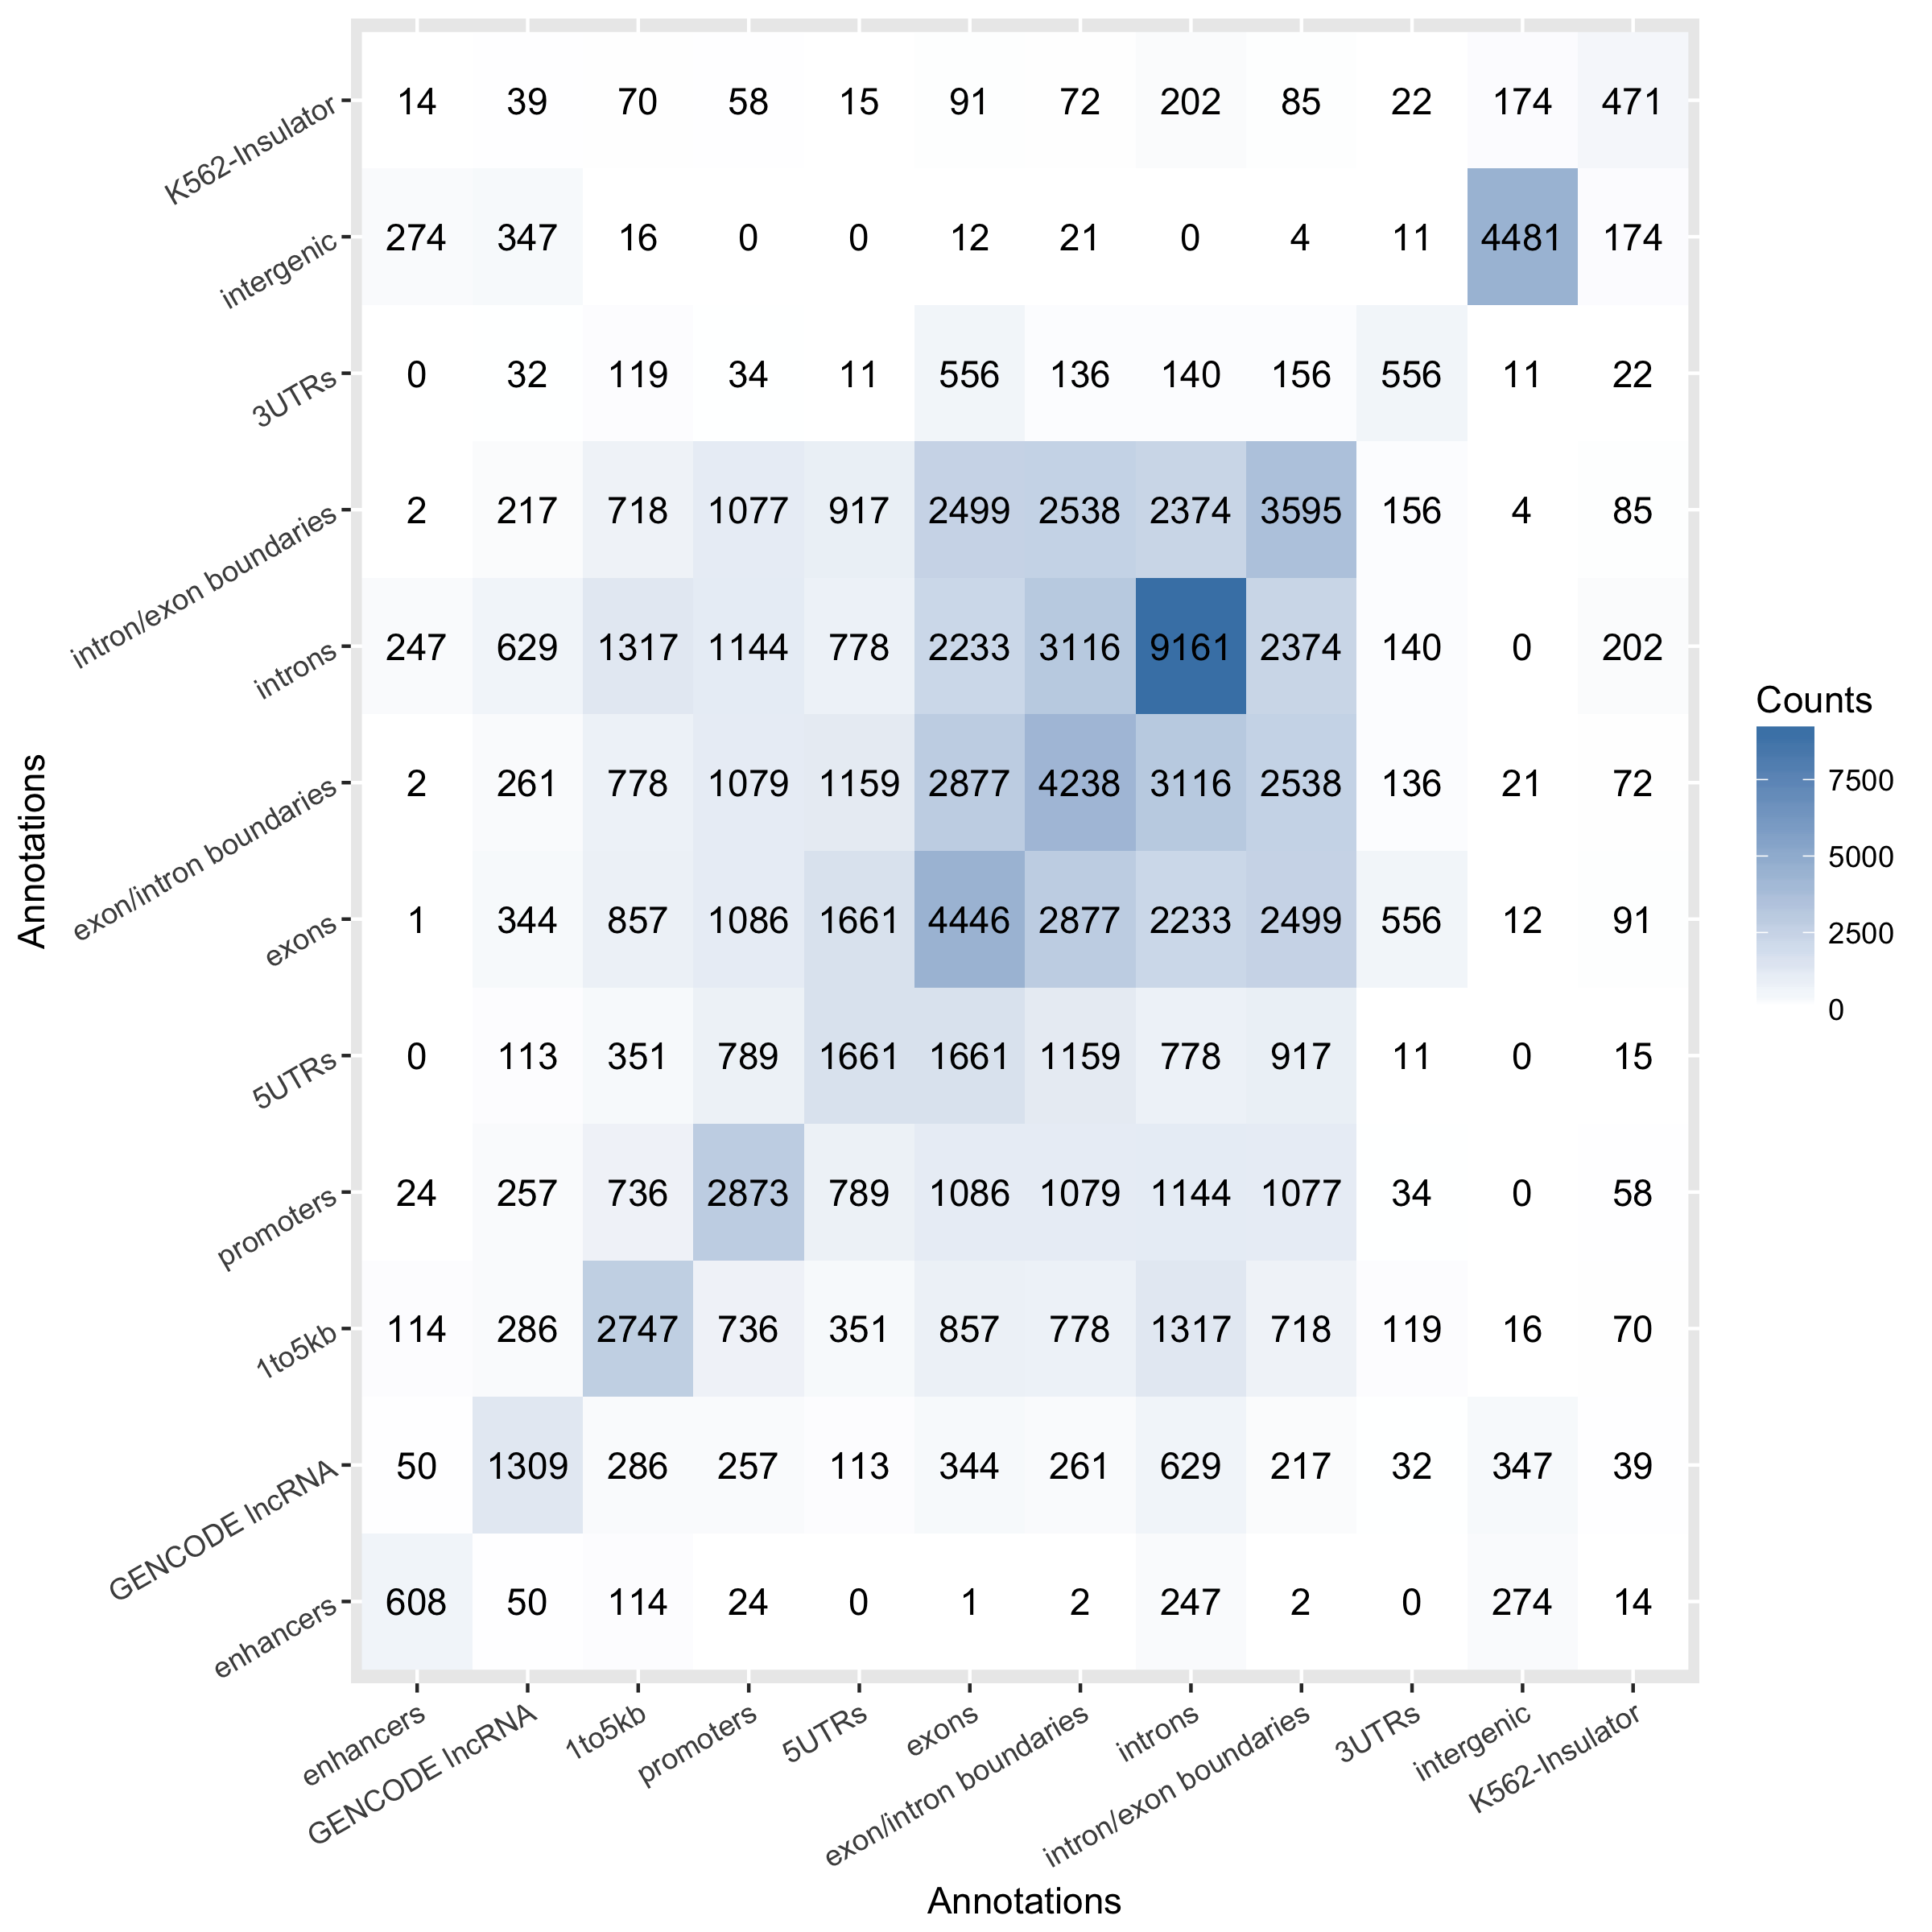
\includegraphics[width=1\textwidth]{chap4figs/figure4_3.png}
\caption[Example of annotatr coannotation heatmap.]
{
% Rackham requires the figure list title matches the first sentence, so repeat that sentence here
\textbf{Example of coannotation heatmap.} The number of input genomic regions occurring in intersections of annotation pairs. This visualization is helpful for prioritizing types of regions to examine in more detail. For example, there are 247 regions that are in an enhancer and reside in an intron.
}
\label{chap4:fig:3}
\end{figure}

\newpage

\begin{figure}[ht!]
\centering
% manually adjust the width of the figure
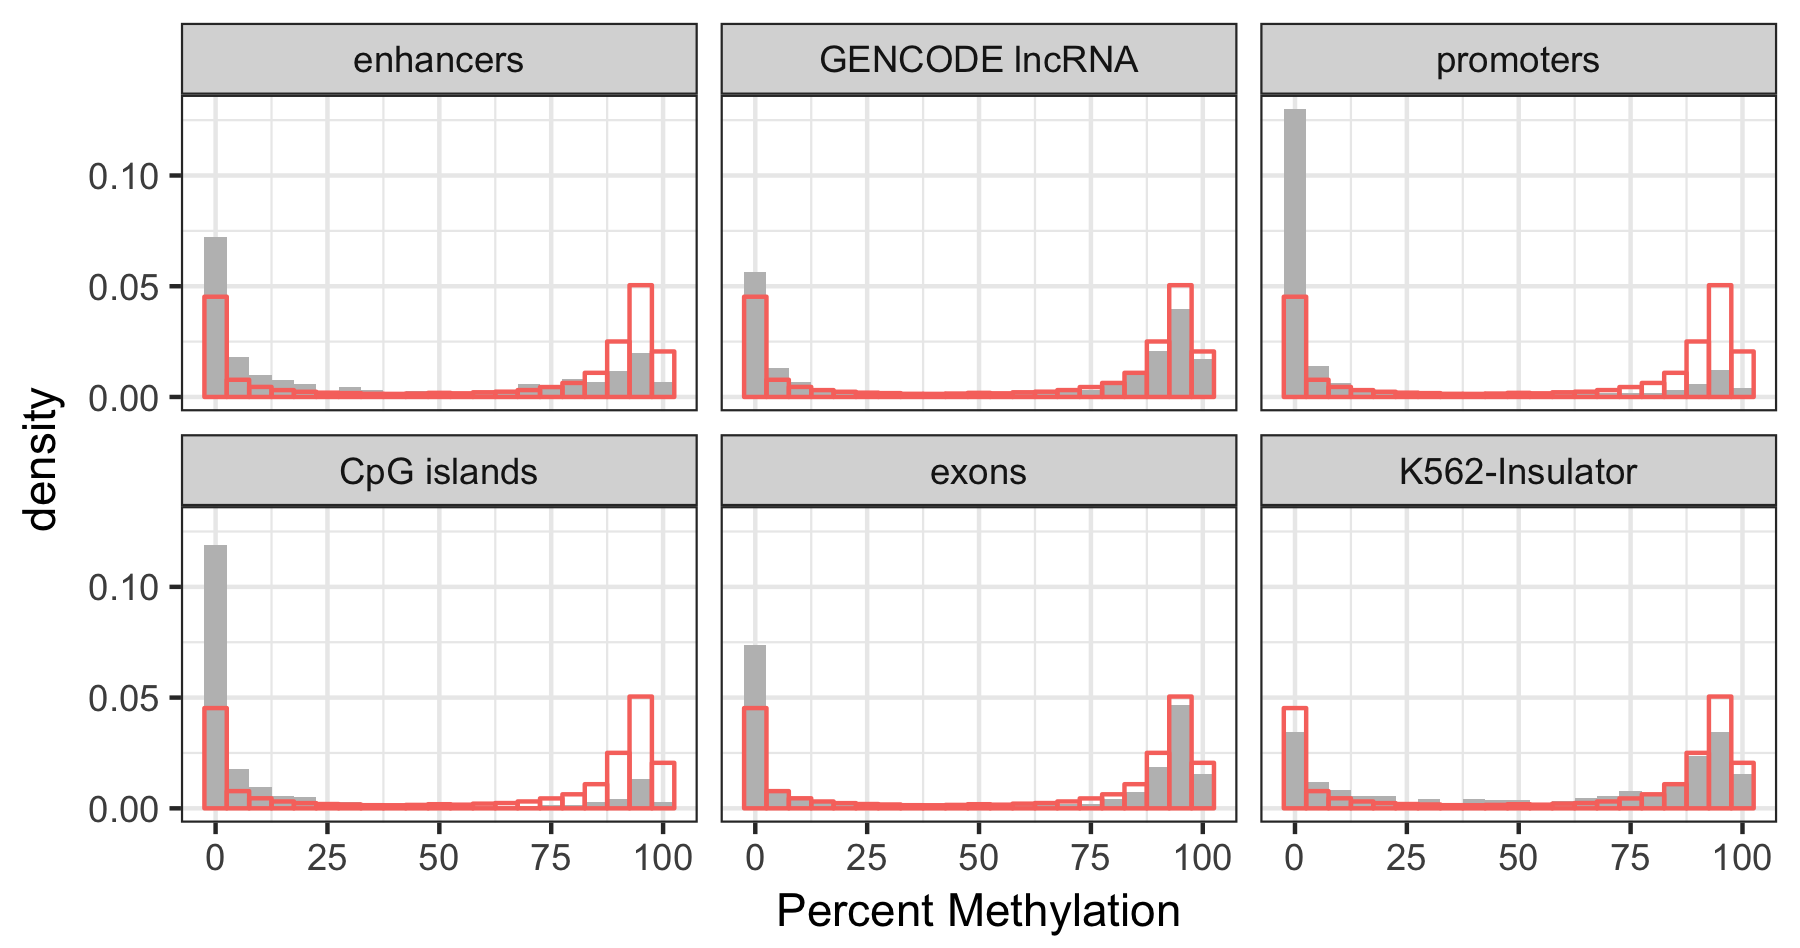
\includegraphics[width=1\textwidth]{chap4figs/figure4_4.png}
\caption[Example of numerical distributions.]
{
% Rackham requires the figure list title matches the first sentence, so repeat that sentence here
\textbf{Example of numerical distributions.} The distribution of the methylation rate across annotations (solid) with the background distribution (outline). Note the clearly visible hyper- and hypo-methylation trends in the different annotation types.
}
\label{chap4:fig:4}
\end{figure}

\newpage

\begin{figure}[ht!]
\centering
% manually adjust the width of the figure
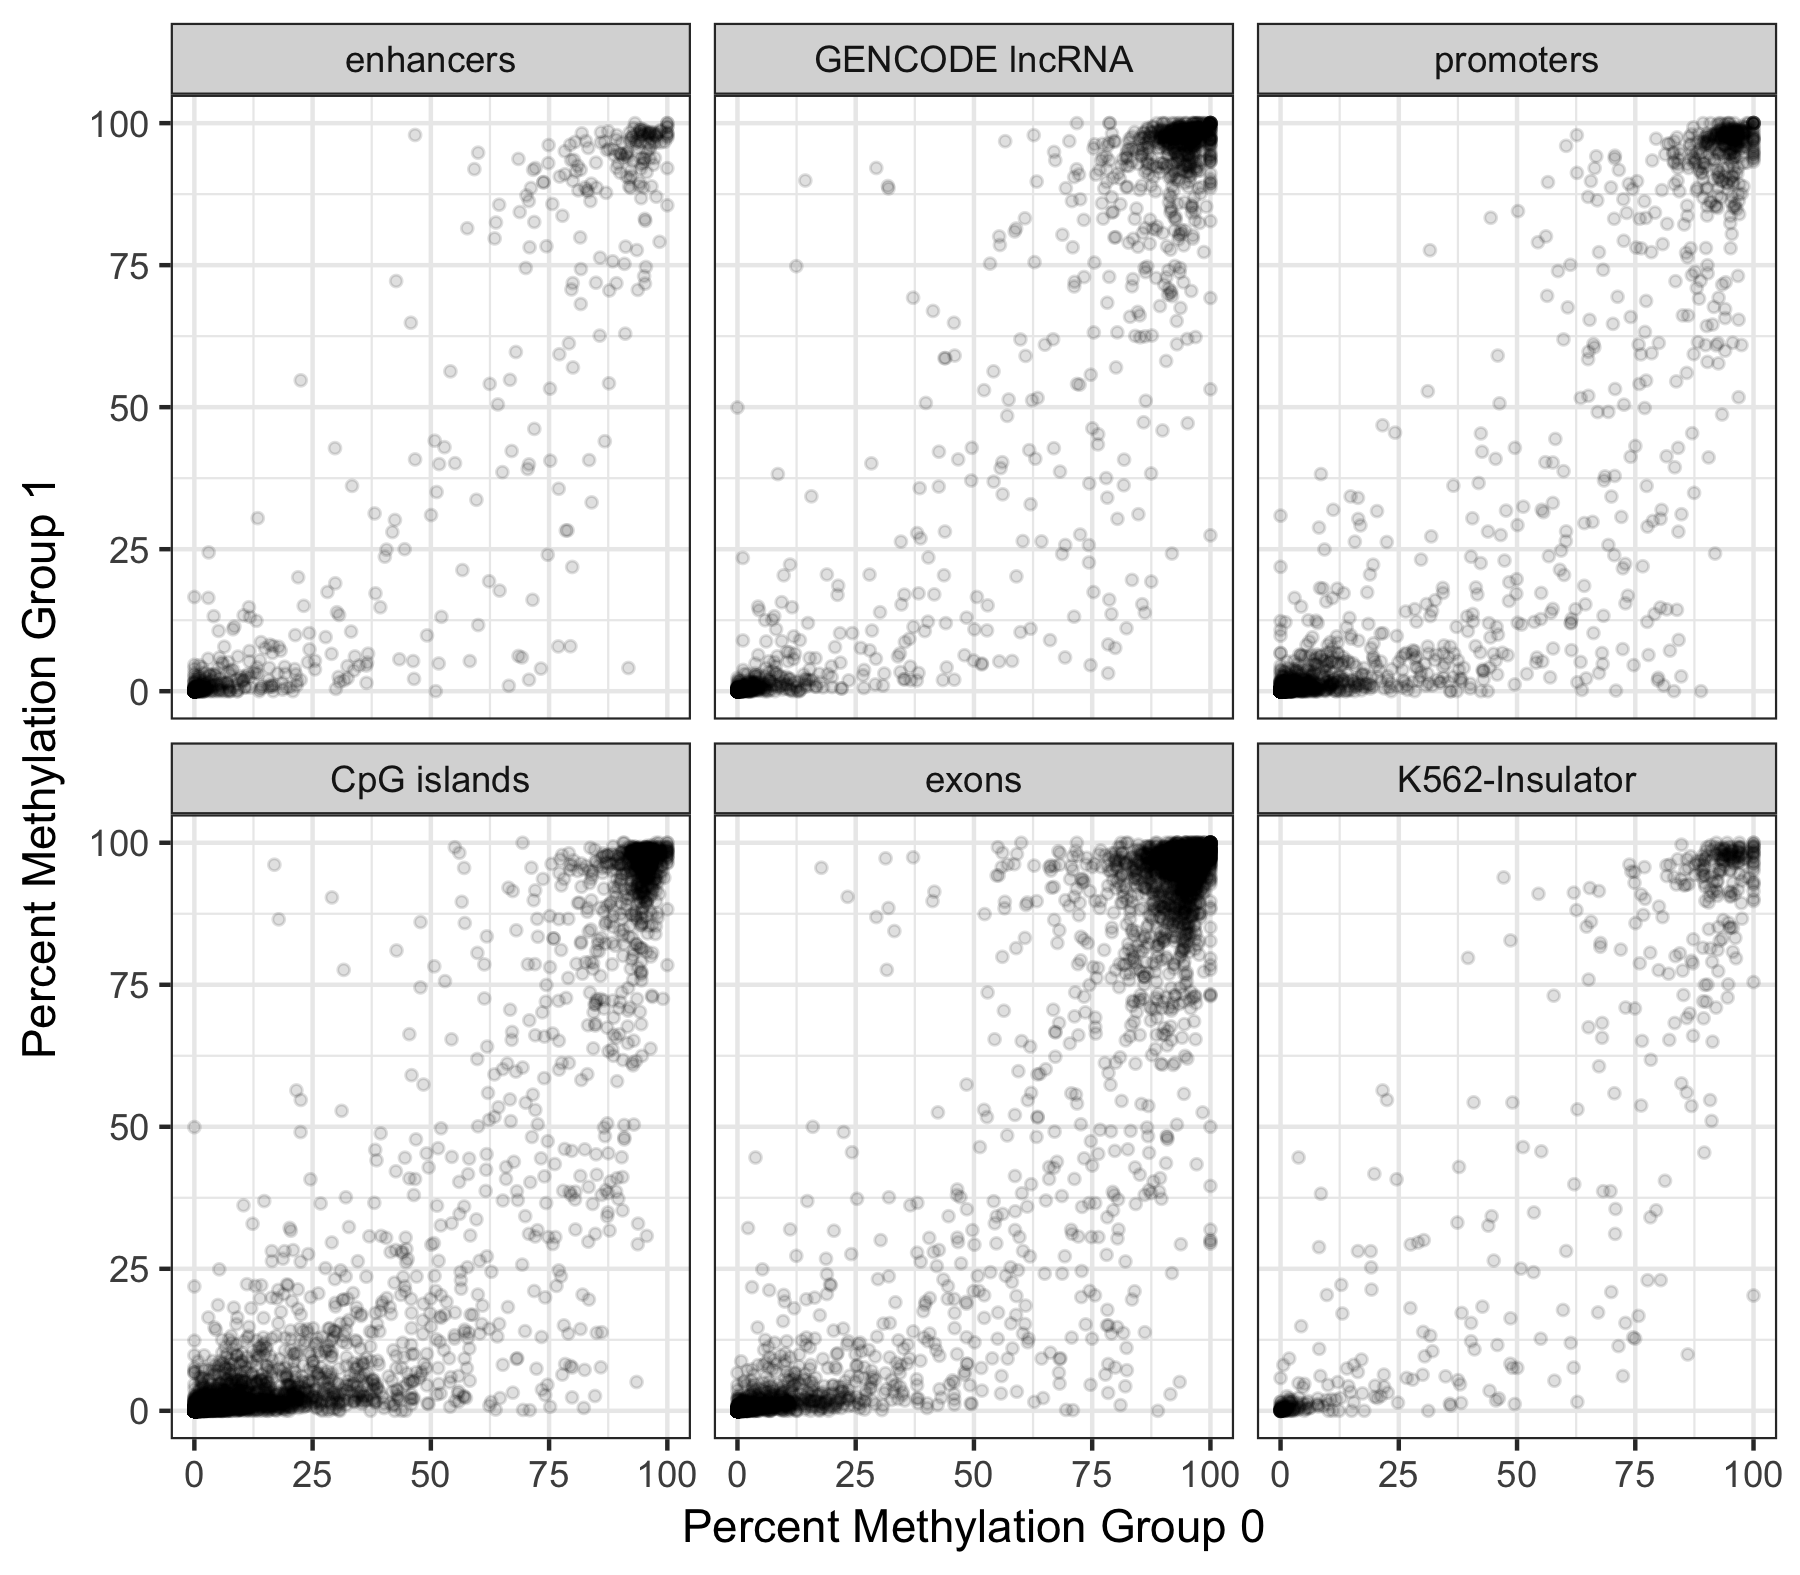
\includegraphics[width=1\textwidth]{chap4figs/figure4_5.png}
\caption[Example of scatterplots.]
{
% Rackham requires the figure list title matches the first sentence, so repeat that sentence here
\textbf{Example of scatterplots.} Scatter plots of methylation rates comparing two sample groups across a subset of the annotation types. This visualization enables quick assessment of correlations in numerical data across different annotations types (or categorical variables).
}
\label{chap4:fig:5}
\end{figure}

\newpage

\begin{figure}[ht!]
\centering
% manually adjust the width of the figure
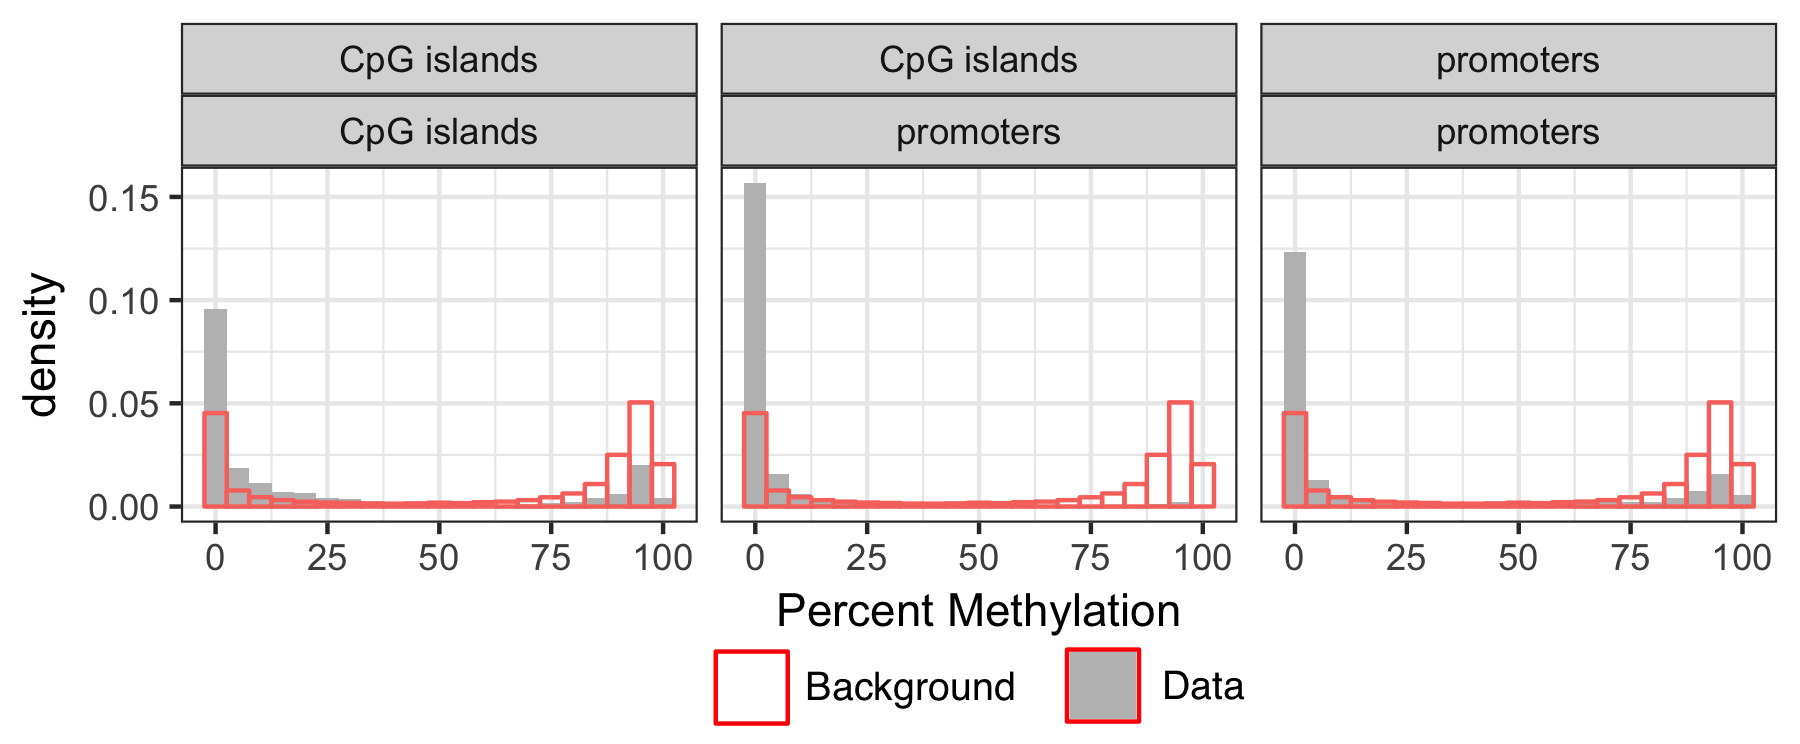
\includegraphics[width=1\textwidth]{chap4figs/figure4_6.png}
\caption[Example of numerical coannotations.]
{
% Rackham requires the figure list title matches the first sentence, so repeat that sentence here
\textbf{Example of numerical coannotations.} The distribution of the methylation rate of regions in just CpG islands (left), promoters and CpG islands (middle), and just promoters (right). Note the relative hypermethylation trend in the co-annotated regions compared to the singly annotated regions.
}
\label{chap4:fig:6}
\end{figure}

\newpage

\begin{figure}[ht!]
\centering
% manually adjust the width of the figure
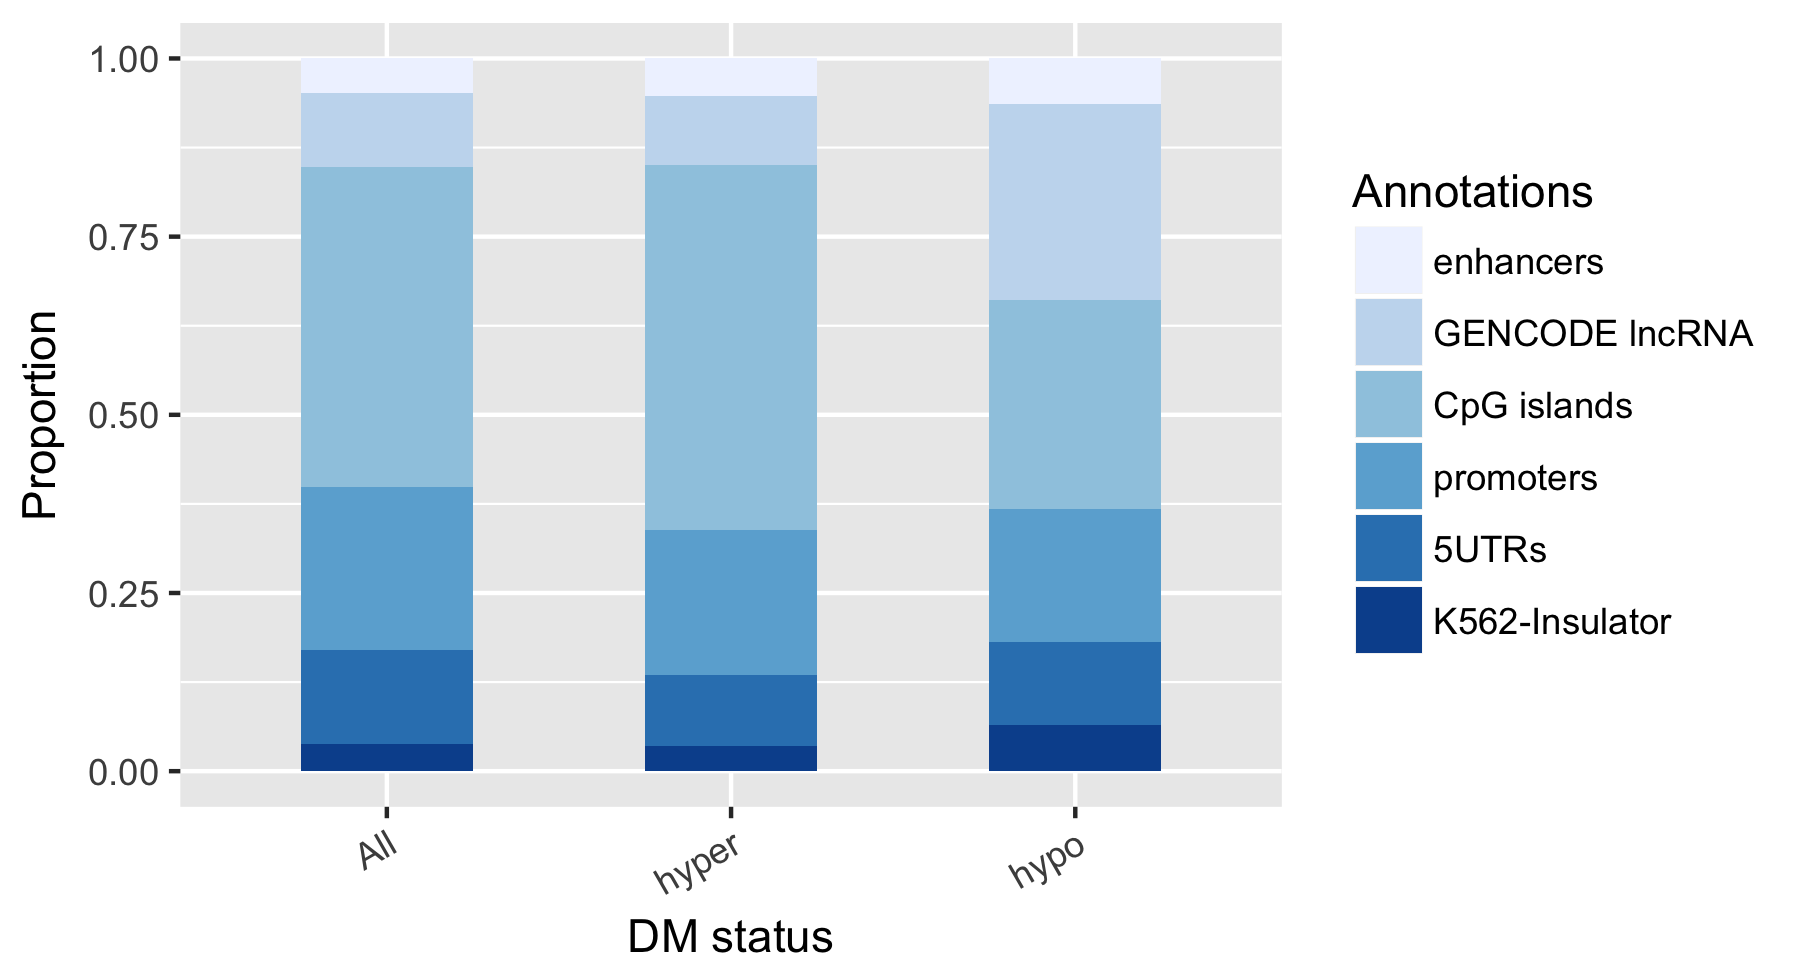
\includegraphics[width=1\textwidth]{chap4figs/figure4_7.png}
\caption[Example of categorical annotations.]
{
% Rackham requires the figure list title matches the first sentence, so repeat that sentence here
\textbf{Example of categorical annotations.} The proportion of annotations of hyper- and hypo-methylated regions, with the background distribution (All) for comparison. Note the differences in enhancers, CpG islands, lncRNAs, and K562-insulators between hyper- and hypo-methylated regions compared to each other and all tested regions.
}
\label{chap4:fig:7}
\end{figure}

\newpage

\begin{figure}[ht!]
\centering
% manually adjust the width of the figure
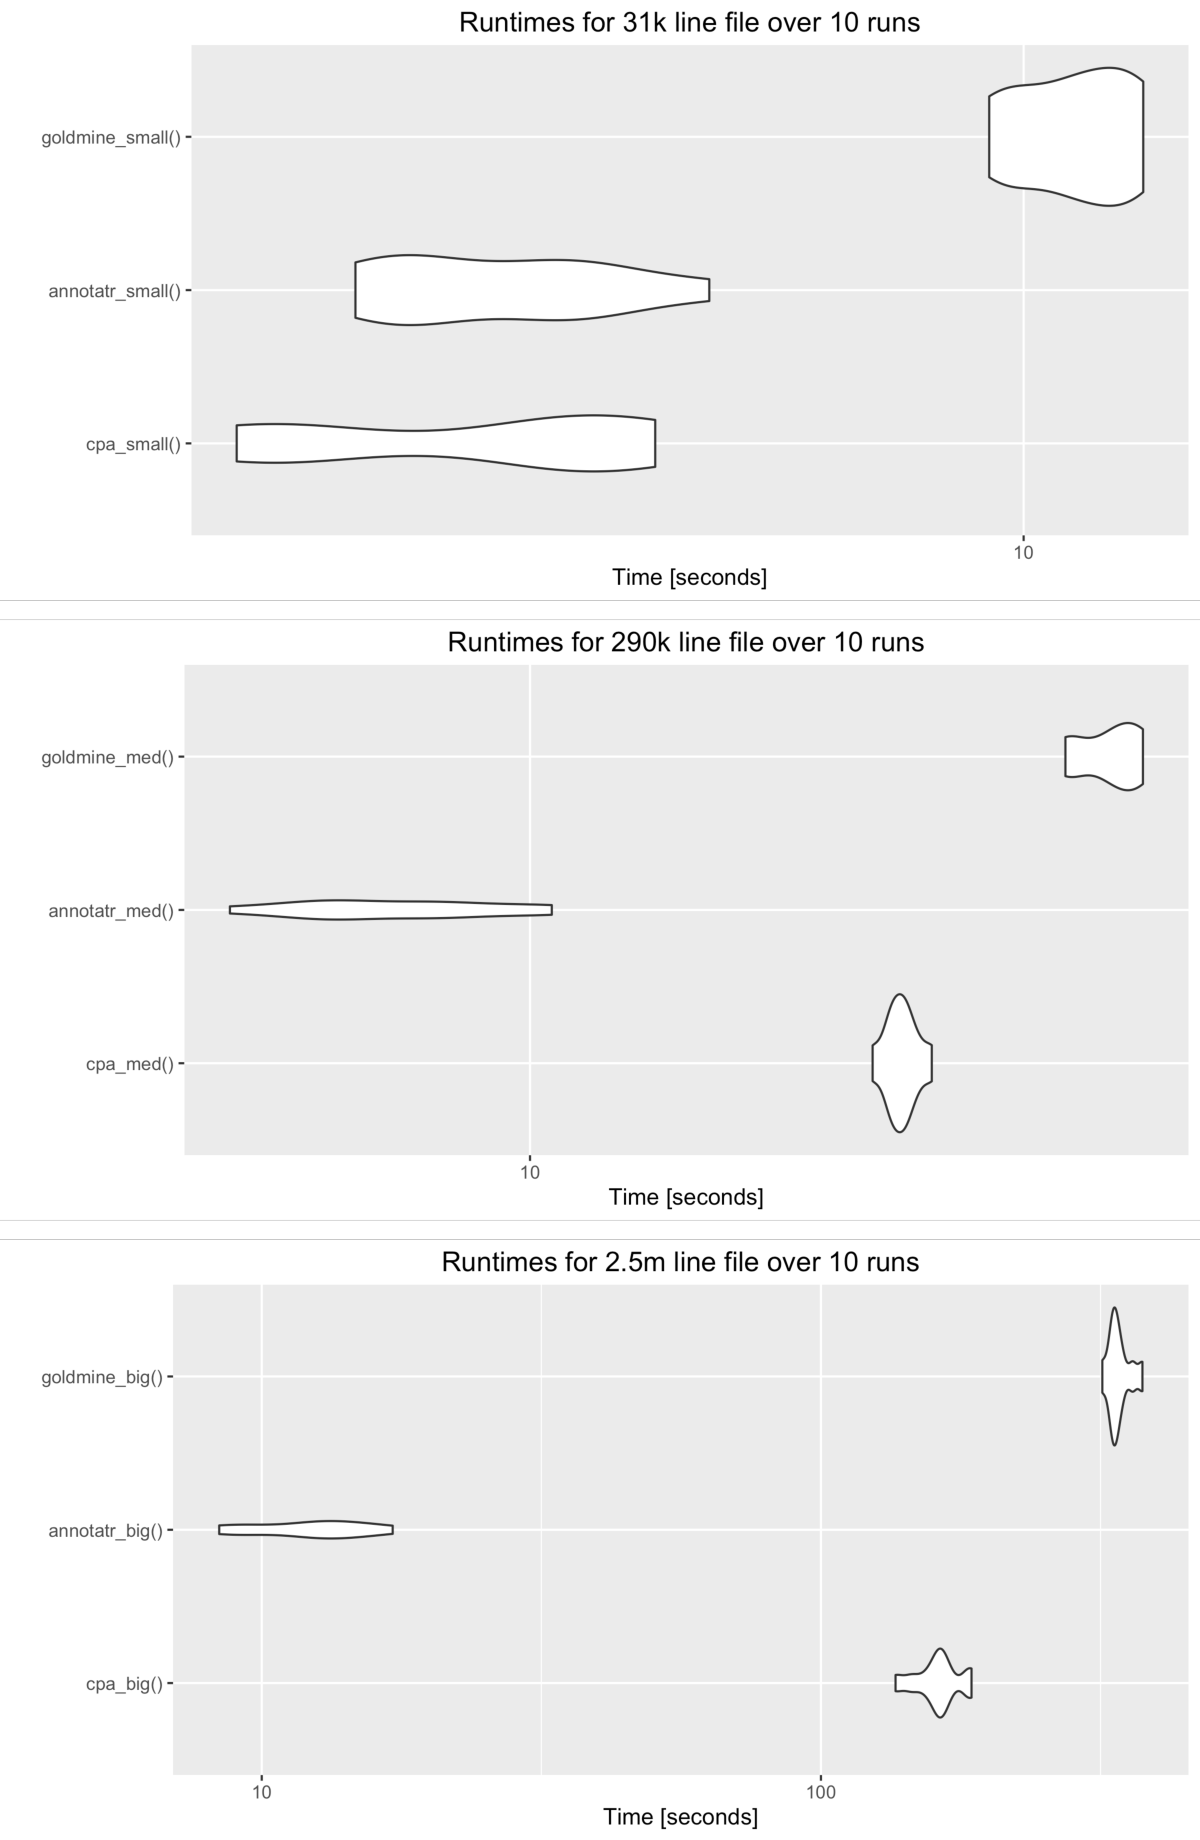
\includegraphics[width=0.8\textwidth]{chap4figs/figure4_8.pdf}
\caption[Benchmarking results for annotatr.]
{
% Rackham requires the figure list title matches the first sentence, so repeat that sentence here
\textbf{Benchmarking results for annotatr.} Violin plots of benchmarking results comparing annotatr to ChIPpeakAnno and goldmine from file read to annotation for small (31k, Top), medium (265k, Middle), and large (2.5m, Bottom) files over 10 runs. Both annotatr and ChIPpeakAnno perform about the same for small files (Top), but for larger files annotatr is clearly faster (Middle) and (Bottom).
}
\label{chap4:fig:8}
\end{figure}
